\chapter{Background}
\label{ch:preliminaries}

In this chapter, we outline the relevant terminology and the theoretical preliminaries that is essential for better understanding of this thesis.
Initially, in Section \ref{sec:bck_rdf_model}, we describe important concepts of RDF as a modeling language and its main serialization formats. 
Next, in Section \ref{sec:bck_parser} discusses parsing techniques and methods to detect and recover syntax errors. Finally, Section \ref{sec:bck_ANTLR} presents an overview of ANTLR framework which is used to automatically generate the internal parser of RDF-Doctor.

\section{The Resource Definition Framework}
\label{sec:bck_rdf_model}

The ``Semantic Web" \cite{W3C:SemanticWebTerm:Online} term  has appeared during the transformation process from ``Web of documents" to ``Web of data", similar to those data found in databases. 
W3C defines it as ``the Web of linked data". 
{Figure \ref{Fig:semanticWebStack}} describes the Semantic Web Stack, proposed by W3C. 
It contains several technologies to enable the users for creating their own data stores on web, building vocabularies and ontologies, as well as enforcing processing rules on such data.   

Subsequently, in order to make data more and more machine-readable and interchangeable between various applications, the RDF model~\cite{W3C:RDF-Primer:Online} has been developed.  
RDF model plays a fundamental role of data exchange in the layered Semantic Web Stack and links the high-level semantic web tools with low-level ones, as illustrated in {Figure \ref{Fig:semanticWebStack}}. 
	\begin{figure}[ht]
	\begin{center}
	\setlength\belowcaptionskip{-7mm}
		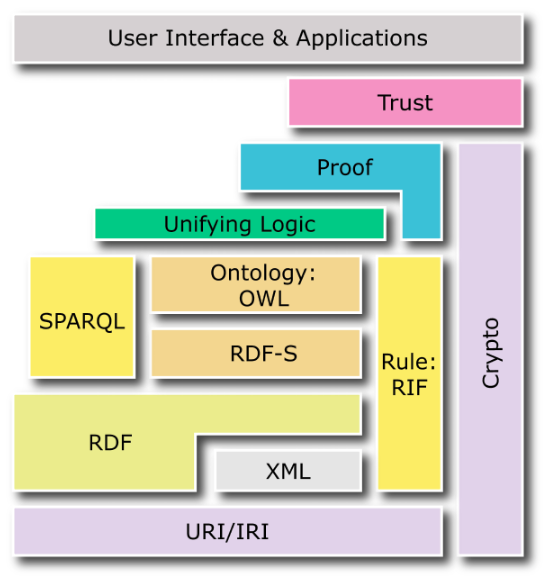
\includegraphics[scale=0.5,angle=0]{images/semanticWebStack}
		\caption{\textbf{Semantic Web Stack \cite{W3C:SemanticStack:Online}.} It is composed of several layers containing different technologies and languages. 
		RDF Model links high-level semantic web tools with low-level ones and works as a bridge to enable data exchange between various applications.}
		\label{Fig:semanticWebStack}
	\end{center}
\end{figure}
\par
Also, {Figure \ref{Fig:rdfModel}}(a) presents a simple graphical depiction of RDF Model. 
A triple is the most atomic unit, which is defined by three main components: a subject, a predicate, and an object. 
It has a common similarity of a basic structure of a simple sentence in a natural language which consists of a subject, a verb, and an object. 
As the verb in natural languages shows a relation and a connection between the other two entities, in the same way in RDF Model, the predicate connects both a subject and an object via a certain property. 

A simple example of modeling a natural sentence using RDF is given in Figure~\ref{Fig:rdfModel}(b). 
It expresses that "Germany has the river Rhein", where \textbf{Ex:Germany} is a subject, \textbf{Ex:hasRiver} is a predicate, and \textbf{"Rhein"} is an object. 
The first two terms uses Uniform Resource Identifiers (URIs) to establish unique identifiers, where \textbf{Ex:} is a declared prefix label in the RDF file to refer to an URI path and the following part \textbf{Germany} is an extension of the path. 
The last value \textbf{"Rhein"} is a literal or a string. %What is given is a simple example of RDF Model to show its fundamental structure, but, in the meanwhile, more examples can be viewed at \cite{W3C:RDF-Primer:Online}.

\begin{figure}[ht]
	\begin{center}
		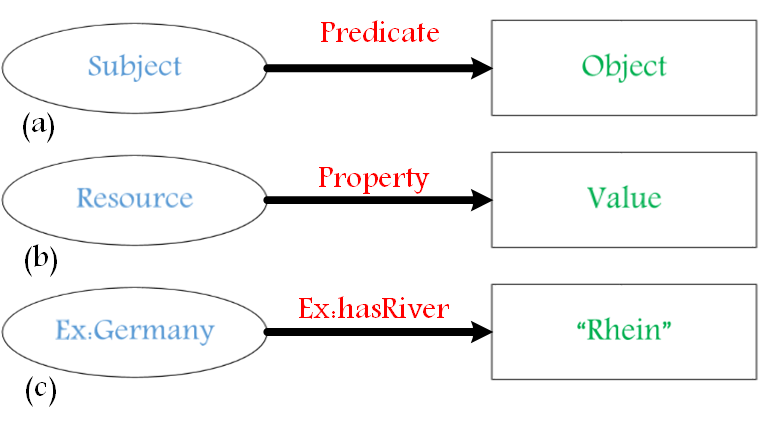
\includegraphics[scale=0.4,angle=0]{images/RDF-Model}
		\setlength\belowcaptionskip{-5mm}
		\caption{\textbf{Graphical representation of RDF model.} A triple is a major component in RDF Model which has a form of Subject-Predicate-Object, as shown by (a), while an example of a natural sentence encoded in the triple format is presented by (b).}
		\label{Fig:rdfModel}
	\end{center}
\end{figure}
RDF data can be represented in a number of different serialization formats.
%as was mentioned in Chapter \ref{ch:introduction} and since their syntax are used as use cases to be parsed with RDF-Doctor , 
In the next two subsections, Turtle and N-Triples are as two common serialization formats. 

\subsection{Turtle Serialization}
Terse RDF Triple Language (Turtle) \cite{W3C:Turtle:Online} is one of the serialization formats, which uses triples for data representation. 
%A triple has Subject-Predicate-Object form, it  has a similarity with some of natural languages where a simple sentence consists of a subject, a verb, and an object. 
In order to understand the syntax of Turtle, some terms  relevant to its syntax are discussed in the following:

\begin{figure}[ht]
	\begin{center}
		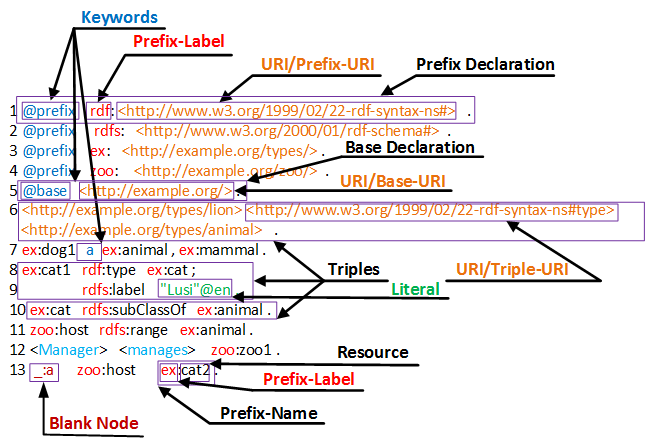
\includegraphics[scale=0.8,angle=0]{images/TurtleStructure.png}
		\setlength\belowcaptionskip{-5mm}
		\caption{\textbf{Structure of Turtle.} Multiple terms represent the syntax of Turtle, they are pointed with one or more matched samples.}
		\label{Fig:TurtleStructure}
	\end{center}
\end{figure}
\begin{itemize}
    \item \textbf{URI\footnote{https://tools.ietf.org/html/rfc3986
}:} refers to a Uniform Resource Identifier, used to point to a web resource, not only a web page address, as a Uniform Resource Locator (URL) do. 
The URI can represented in the following forms: 1) Absolute form (similar to URL in-between 2 brackets, lines 1 and 6, pointers show samples of absolute URIs); 
2) Relative form or \textbf{Relative URI}, this form is used when a base URI is defined, line 5 shows a declaration of a base URI, then, line 12 shows two samples of relative URIs, i.e., \textless Manager\textgreater and \textless manages\textgreater; and 
3) Short form (referred as \textbf{Prefixed-Name} and discussed next).
  \item \textbf{Prefix:} a prefix declaration is a shortcut way to replace absolute URIs with abbreviated ones. Essentially, it contains a \textbf{Prefix-Label} and \textbf{Prefix-URI}. 
  Prefix samples are shown in the first four lines of Figure \ref{Fig:TurtleStructure}, starting with \textbf{@prefix} keyword, followed by a \textbf{Prefix-Label}, then a colon, next comes a URI or a \textbf{Prefix-URI}, and lastly, an end dot. 
 \item \textbf{Prefix-Name:} a short URI consists of a \textbf{Prefix-Label}, followed by a colon, then a resource name. An example is illustrated in line 13.
        
  \item \textbf{Prefix-Label:} a short sequence of characters to avoid re-writing of a long absolute URI.
  \item \textbf{Prefix-URI:} an absolute URI is used in prefix declarations. 
  \item \textbf{Base:} a declaration to define a base URI used inside a Turtle file. 
  This could be also another shortcut form for URIs when they have a common path, then the last local part in URIs can be written inside 2 brackets. 
        
\item \textbf{Directive:} prefix and base declarations can be considered as directives, similar to those declarations of libraries in common programming languages.  
    \item \textbf{Blank Node:} an identifier for a temporal or unnamed resource~\cite{journals:tkde:GutierrezHV07}, it starts with ":\_", then a sequence of characters (referred as BlankNode-Label). 
    Figure \ref{Fig:TurtleStructure} line 13 shows a blank node in the position of Subject.  
    \item \textbf{Literal:} a string, a date, a numeric or a boolean value as shown in line 9.
\end{itemize} 

The main components in Turtle syntax are prefixes and triples. 
Prefixes are used to make Turtle a user-friendly language and to reduce the redundancy of repeating absolute URI, subject, and subjects and predicates, if one subject or one predicate are shared together on more than one object. 

\begin{figure}[ht]
	\begin{center}
		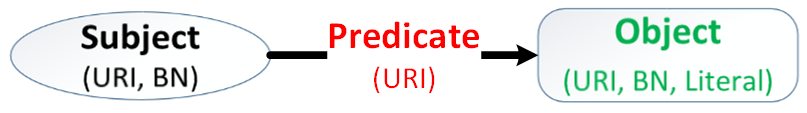
\includegraphics[scale=0.4,angle=0]{images/TurtleandNtripleElements.png}
				\setlength\belowcaptionskip{-5mm}
		\caption{\textbf{ Elements of triples in Turtle and N-Triple serializations.} A triple consist of a Subject, a Predicate, and an Object. A Subject can be either URI or Blank Node (BN), a Predicate is only URI, while an Object can take URI, BN or Literal forms.}
		\label{Fig:TurtleandNtripleElements}
	\end{center}
\end{figure}

In the following, the basic rules defined in the Turtle serialization are outlined:

\begin{itemize}
    \item Each directive (a declaration of Prefix or Base) or triple ends with a dot.
    \item Figure \ref{Fig:TurtleandNtripleElements} shows elements of a triple and their possible forms, as follows: \textbf{Subject} can be either a blank node, or URI, a \textbf{Predicate} is only URI, and an \textbf{Object} can be either an URI, a Literal or a blank node.
    \item When multiple \textbf{Objects} share the same \textbf{Subject} and \textbf{Predicate}, then comma separates between those \textbf{Objects}.
    As example is demonstrated in Figure \ref{Fig:TurtleStructure} line 7 where both \textbf{ex:animal} and \textbf{ex:mammal} have the same subject \textbf{ex:dog1} and the same predicate \textbf{a} (a keyword substitutes the \textbf{rdf:type} term) and are separated by a comma.
    
     \item A semicolon separates combinations of a \textbf{Predicate} and an \textbf{Object} when these combinations share the same \textbf{Subject}. 
     Both lines 8 and 9 of Figure \ref{Fig:TurtleStructure} shows this pattern where a combination of a predicate \textbf{rdf:type} and an object \textbf{ex:cat} and the other combination of the predicate \textbf{rdfs:label} and the object \textbf{"Lusi"@en}, share the same subject \textbf{ex:cat1}, and they are separated by a semicolon.
     
      \item Prefix and Base declarations are commonly written on the top of Turtle files or at least before the first use of them in a Turtle Document.
      
     \item Literals are strings or numbers. 
     Strings have multiple forms: 1) a string in single line, written between two single or double quotes; 2) a string in multiple lines, starts with three single or double quotes and ends with the same number of quotes; 3) a string with a language tag, has one of the previous two forms, and is followed by language tag, i.e., \textbf{@} which contains a few sequence of characters to identify the language of the preceding string; and 4) a string with a certain data-type, again has one of the first two forms, followed by \textbf{\textasciicircum\textasciicircum}, associated with a data-type URI, as for example \textbf{``Lusi"\textasciicircum\textasciicircum\textless http://www.w3.org/2001/XMLSchema\#string\textgreater} is a string sample of XML Schema data-type~\footnote{\url{https://www.w3.org/TR/xmlschema11-2}}.
     In addition it can contain numbers, such as decimals, integers, doubles or boolean values, i.e., \emph{true} or \emph{false}.
     \item Blank Node identifier refers one or more triples with no persistent URI and must use the same identifier in the whole Turtle file.   
     
     
\end{itemize} 

\subsection{N-Triple Serialization}
N-Triples \cite{W3C:Ntriples:Online} is the simplest serialization format that organizes RDF data in a form of triples, however, it is hard to be read by users, since long absolute URIs are mostly used to represent \textbf{Subjects}, \textbf{Predicates}, and \textbf{Objects}. 
Figure \ref{Fig:NTriplesStructure} shows an N-Triple example where the only three following elements are serialized: \textbf{Absolute URIs}; \textbf{Blank Nodes}; and \textbf{Literals}. 

N-Triple is considered as a subset of Turtle serialization. 
Additionally, its content formed by \textbf{Subjects}, \textbf{Predicates}, and \textbf{Objects} is shown in Figure \ref{Fig:TurtleandNtripleElements}, which is quite similar to Turtle, however, a type of absolute URIs is only used in N-Triple. 
So, N-Triples has no prefix or base declarations, and repeats subjects even if they are shared from predicates and objects. Furthermore, a general form of N-Triples can be reached,  consisting of a \textbf{Subject}, followed by a \textbf{Predicate}, next comes an \textbf{Object}, finally, it ends with \textbf{a dot}.   

\begin{figure}[ht]
	\begin{center}
		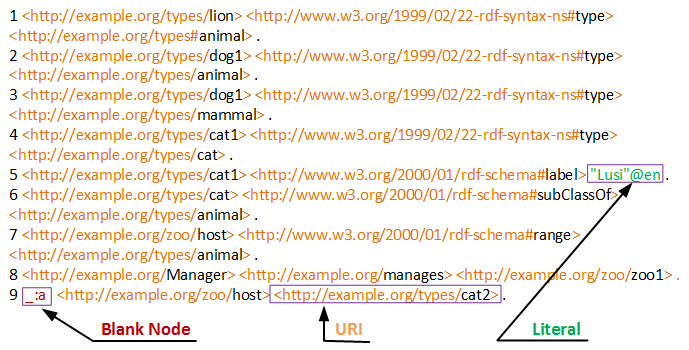
\includegraphics[scale=0.8,angle=0]{images/NTriplesStructure.png}
		\setlength\belowcaptionskip{-5mm}
		\caption{\textbf{Structure of N-Triple serialization.} 
		Main elements of N-Triple serialization are URIs, Blank Nodes, and Literals. 
		The URIs of local terms or resources defined within an N-Triple document are colored in black.}
		\label{Fig:NTriplesStructure}
	\end{center}
\end{figure}


\section{Parsing and Error Recovery}
\label{sec:bck_parser}
This section discusses the role of the parser in the compiler, various types of parser developments, and lists the methodologies for error recovery. 

\subsection{Parsing and Grammar Definitions}

%It is of great benefit to shed a light on parsing term to understand later the approach of this study. 
In \cite{parsingGuide2017}, Gabriele Tomassetti has defined \textbf{parsing} as:{\it  \textbf{``the analysis of an input to organize the data according to the rule of a grammar''}}. It can be intelligibly recognized that parsing deals with some input data and tries to analyze it based on a given grammar. 
On the other hand, a \textbf{grammar} is defined by ~\cite{parsingGuide2017} as {\it \textbf{``a formal grammar is a set of rules that describes syntactically a language''}}. 
According to this definition, rules are a crucial component of the grammar used to define the syntax of a language.

\subsection{The Role of in Compilers}
A parser is an essential element in  compilers. 
{Figure \ref{Fig:parserPosition}} illustrates the role of the parser in a compiler. 
The first component ``Lexical Analyzer" receives the input data, then produces tokens for the ``Parser" component. Parser constructs a \emph{parse tree} based on its grammar rules and continues to process every token until it consumes all the tokens. 
The parse tree as an output of the parser is delivered to the next phases of the compiler. 
In general there a two groups of errors, lexical errors mainly generated by Lexical Analyzer while syntax and semantic errors generated by Parser.
%TODO{add the ref or change the image}

\begin{figure}[ht]
	\begin{center}	\setlength\belowcaptionskip{-5mm}
	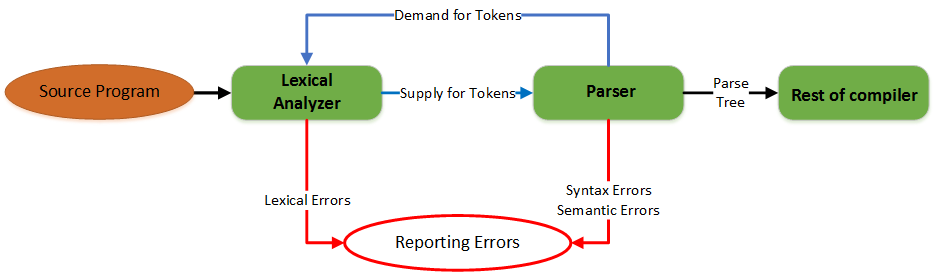
\includegraphics[scale=0.55,angle=0]{images/ParserRole}
	\caption{\textbf{Parsing process \citep{JCOMP:Tool:Online}}. 
	A parsing process has two main components: a Lexical Analyzer and a Parser. 
	The Lexical Analyzer supplies input tokens to the Parser.
	Once it has enough tokens, the Parser starts parsing the supplied tokens, then it requests again new tokens from the Lexical Analyzer, and this step continues until reaching the end of file symbol (announcing the end of tokens).	Any lexical error is generated by the Lexical Analyzer whereas syntax and semantic errors are produced by the Parser.
	In the end, a parse tree containing information about parsing process is produced.}
		\label{Fig:parserPosition}
	\end{center}
\end{figure}

\subsection{Parser Developments}
In order to build a parser, there are two available options, either by starting to code your own parser or getting an off-the-shelf automatic parser generator tool to automatically create the parser source code from a grammar file. 
In the following, both approaches are outlined:

\textbf{1) Writing a parser source code from scratch:} this means, a developer has to write and implement all necessary components, including the lexical analyzer and the parser classes. 
On the one hand, this way gives more flexibility in handling several issues, triggered when dealing with certain token patterns, such as special characters and escape sequences. 
On the other hand, it consumes much time and requires a large amounts of efforts.

\textbf{2) Generating a parser source code using automatic parser generators:} a parser generator outputs the desired parser source code. 
Predominately, such tools can be used to do a specific parsing task, but again, a grammar identifying a particular syntax is required as an input for those tools. 
The main benefit here is the less time and effort needed to build a parser.
The flexibility is reduced to the features and classes provided by those tools.
Otherwise, such flexibility can be optimized by implementing new classes and modules on top of existing ones with the objective of dealing with specific cases, for example to parse a large file, which frequently, an "full memory space" error is encountered.
This case can be solved by adding a class that divides a large file into chunks to be sequentially parsed.  

\subsection{Error Recovery Methodologies in Parsers}
In any parser, the error recovery techniques specify the its behavior with dealing with errors once they are detected.  
Aho et al \cite{Aho:2006}, have outlined such techniques as follows:

\begin{itemize}
	\item \textbf{Panic-Mode Recovery}: once an error has been discovered, the parser ignores and skips to next input symbols, one by one till a recognized set of tokens is detected. 
	In spite of discarding of huge number of input symbols without checking them for further error detection, it is considered a simple parsing mode and do not fall in an infinite loop while other modes may do.
	
	\item \textbf{Phrase-Level Recovery}: to continue the parsing process, the parser performs local correction. A typical local correction in RDF data, for example, is to insert a missing dot or delete extraneous dots.
	
	\item \textbf{Error Productions}: by expecting common and well-known errors, production rules can be inserted into the grammar. 
	Then, the generated parser is well-informed about such errors. 
	Error detection and error recovery is easily realized in this case, where error details are controlled by the developer, such as the error location, the exact type of error, etc. 
	Furthermore, a customized and meaningful error message for the identified error can be provided as well. 
	
	\item \textbf{Global Correction}: conventionally, the parser tries to reduce as much as possible number of change operations (such as, insertion, deletion and modification), when dealing with an incorrect input token with the objective of lowering the total cost of error correction. 
	To make it more clear, let us assume an incorrect input statement X is given in a grammar G, the parser constructs a closest error-free parse tree of a statement Y to replace the statement X, such that the changes are as small as possible. 
\end{itemize}


\section{ANTLR Parser Generator}
%The parser module in RDF-Doctor was automatically built with a help of ANTLR Parser Generator based on our grammar as an input, as well as,  the ANTLR library is used as a plug-in. 
In the following text, a short overview of ANTLR and its generation process of a parser are discussed.   
\label{sec:bck_ANTLR}

\subsection{ANTLR in a Nutshell }
ANTLR is a useful and easy to use tool for the purpose of creating of dedicated parsers for specific domain languages. 
It enables an automatic generation of a source code for a parser with less time and effort. 
The core requirement of ANTLR is the definition of a syntax grammar for a desired language. 
The grammar contains language rules used to model the syntax and the semantic of the given language for which the parser will be built. 

\subsection{ANTLR as a Parser Generator}
As already has been discussed, the compiler has two main components: a Lexical Analyzer (called also Lexer) and a Parser. 
Both Lexer and Parser are needed to have their rules defined in the grammar file. 
Lexer rules are those rules used to construct the terminals, whereas Parser rules determine the non-terminals. 
Another essential point is the process of parser creation as demonstrated in Figure~\ref{Fig:ANTLR}, where the parser program is generated with the help of ANTLR framework. 
In more details, the parsing process is based on ~\cite{ANTLR:Tool:Online}, which starts the required grammar and ends with the output of the parse tree:

\begin{figure}[ht]
	\begin{center}
		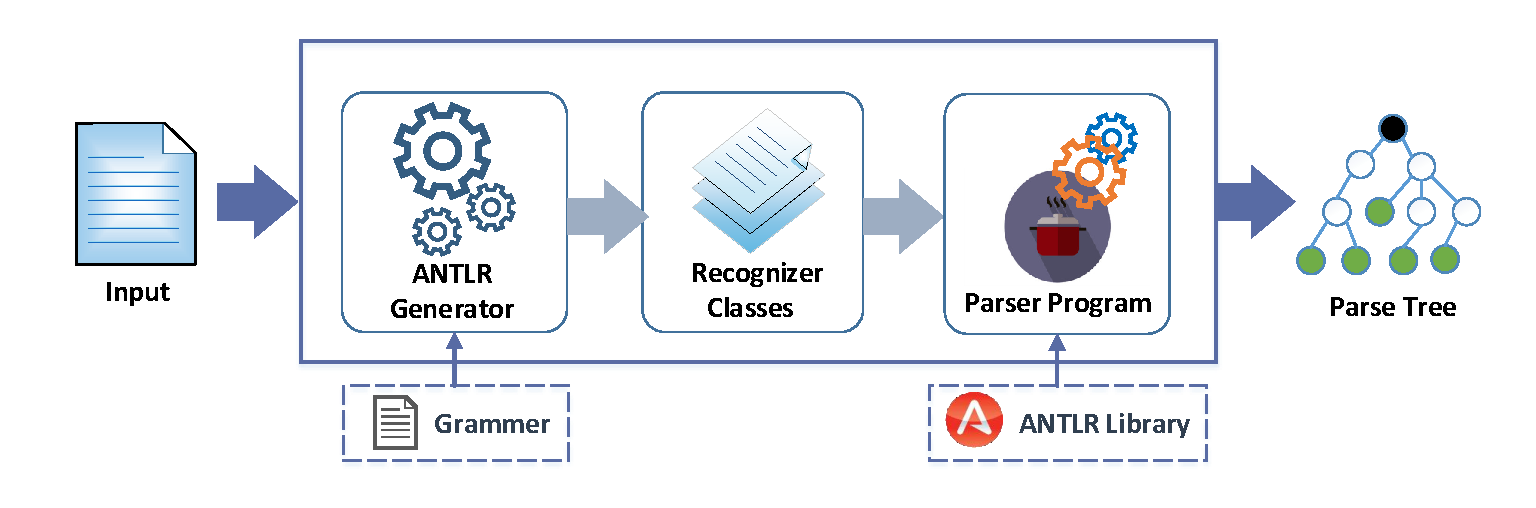
\includegraphics[scale=0.52]{images/ANTLR.pdf}
				\setlength\belowcaptionskip{-5mm}
		\caption{\textbf{Parsing process based on ANTLR parser generator\cite{ANTLR:Tool:Online}.} 
		ANTLR parser generator receives the grammar file to generate the classes of the Lexer and the Parser.
		Once the input text is submitted, the generated classes using of ANTLR library are enabled to start the parsing process and generate the parse tree.}
		\label{Fig:ANTLR}
	\end{center}
\end{figure}


\begin{enumerate}
		\item  {\bf Writing a grammar file:} commonly, a grammar called a \emph{Parsing Expression Grammar} (PEG) is required to build a parser. 
		ANTLR requires a context-free grammar, crafted with the Extended Backus-Naur Form (EBNF). 
		EBNF consists of a sequence of rules which describe the syntax and the semantic of an input which needs to be parsed. 
		Both terminals or non-terminals are types of head rules. 
		On the one hand, terminals are leaf elements with no grammatical structure, e.g., words or numbers. On the other hand, non-terminals have a definite grammatical structure and name, e.g., triples or prefixes. 

		\item {\bf Generation of recognizer target\_based classes by ANTLR:} a crucial feature of ANTLR is its capability of automatic generation of the parser source code for a variety of the programming languages like \cite{ANTLR:Website:Online}: Java, C\#, Python (2 and 3), JavaScript, Go, C++, and Swift.
		
		\item {\bf Feeding an input file for parsing:} as an input, ANTLR can parse text documents without additional libraries. 
		Users send their input files for parsing where the parsing process will be achieved based on the crafted grammar in the first step.
		
		\item {\bf Parsing procedure:} {Figure \ref{Fig:ANTLR} } illustrates this step as a cooking phase. 
		In this step, all materials and ingredients are available. 
		The materials are: 1) the auto-generated parser, and 2) the ANTLR library. 
		The ingredients are one or more text files to be parsed. 
		
		\item {\bf Delivering of a final report and a parse tree as an output:} now, the final result is ready.
		All produced output from this process, containing of a parse tree and a report of collected errors is given to the user.
	\end{enumerate}











